\subsubsection{Dynamic Programming Mehtod}
\label{lab:DynamicProgrammingEquation}

\textbf{
Although solving the ILP formulation will result in an “optimal” node mapping, its exponential time complexity makes such approach impractical for large quantity of virtual nodes situation. In this section, we describe an alternative using dynamic programming heuristic that has only a polynomial time complexity and, thus, is feasible for large quantity of virtual nodes situation.
}
\textbf{
To describe the proposed $\MyAlgorithmMethodAbrreviation$ algorithm based on dynamic programming, let us number the virtual nodes from 0 to n, where n is the number of virtual network request node. In addition, let $dp[i][{x_1}][{x_2}] \ldots [{x_m}]$ be the “best” node's placement (place virtual node onto qualified physical node so as to minimize total weight sum) to place the i-th virtual node with the former i-1 virtual nodes were optimal to be placed and node computation up-bound capacity (the node computing sum of all virtual node which is mapped onto this physical node less than the physical node's node computing capacity) of every physical node is $x_1,x_2,\ldots,x_n$, respectively.  The pseudo-code of the dynamic programming based algorithm is shown in Alg.\ref{alg:DPAlg}, and take out a simple example as shown in Fig.\ref{fig:DPIllustration}.
}



\textbf{
As shown in Fig.\ref{fig:DPIllustration} Line 1, when optimal weight sum of placing the first node $v_1$ with node computation capacity of the first and second physical node is 0 and 2 respectively is calculated from not placing any virtual node with node computation capacity of the first and second physical node is 0 and 0 respectively.
}

\textbf{
As shown in Fig.\ref{fig:DPIllustration} Line 2 and Line 3, when optimal weight sum of placing the first node $v_2$ with node computation capacity of the first and second physical node is 2 and 3 respectively is calculated   from the minimum of between placed former 1 node with node computation capacity of the first and second physical node is 1 and 3 respectively, and placed former 1 node with node computation capacity of the first and second physical node is 2 and 2 respectively.
}

\textbf{
As shown in Fig.\ref{fig:DPIllustration} Line 4, when optimal weight sum of placing the first node $v_2$ with node computation capacity of the first and second physical node is 3 and 0 respectively is only calculated   from the minimum of between placed former 1 node with node computation capacity of the first and second physical node is 2 and 0 respectively.
}

\textbf{
As shown in Fig.\ref{fig:DPIllustration} Line 6, when optimal weight sum of placing the first node $v_3$ with node computation capacity of the first and second physical node is 4 and 4 respectively is only calculated from the minimum of between placed former 2 nodes with node computation capacity of the first and second physical node is 2 and 4 respectively, because virtual node $v_3$ must be placed onto first physical node ($f_1\in F_1,f_1\notin F_2$).
}

\textbf{there are n+1 level's dynamic programming functions and there are $\prod_{i=1}^{m}C^i$ dynamic programming functions in every level. The time complexity of calculating every dynamic programming function is $O(m)$. Therefore, overall time complexity of the dynamic programming method is $n*\prod_{i=1}^{m}C^i*O(m)=O(n*m*\prod_{i=1}^{m}C^i)$. Additionally, for recording every level's virtual node's placement, the overall space complexity is $O[(n+1)*\prod_{i=1}^{m}C^i]$, which is, however, could be optimized to $O[\prod_{i=1}^{m}C^i]$, because when updating every level's dynamic programming function, the dynamic programming function only use back step level's dynamic programming function.}


Placing the i-th virtual node where node computation capacity of every physical node is $x_1,x_2,x_3$, the optimal result $dp[i][{x_1}][{x_2}][{x_3}]$ is inferred from the optimal result of the former i-1 virtual nodes are succeed to be placed. For example, for requesting $dp[i][{x_1}][{x_2}][{x_3}]$, the state is inferred from $dp[i-1][{x_1-d_i}][{x_2}][{x_3}]$ when former i-1 virtual nodes are succeed to be placed and node computation capacity of every physical node is $x_1-d_i,x_2,\ldots,x_n$. The state of $dp[i-1][{x_1-d_i}][{x_2}][{x_3}]$ is optimal result when calculating $dp[i-1][{x_1-d_i}][{x_2}][{x_3}]$, and first physical node's node computation capacity $x_1-d_i+d_i$  of $dp[i][{x_1}][{x_2}][{x_3}]$ add $d_i$ because the i-th virtual node is placed into the first physical node.


The formulation of our survivable virtual network embedding problem is standard multiple knapsack problem's formulation, we propose a dynamic programming method for solving the multiple knapsack problem. Assume $C_1,C_2,\ldots,C_n$, $C_i$ are strictly positive integers. Define dynamic programming function $dp[i][{C_1}][{C_2}] \ldots [{C_m}]=0(C_1\leq c_1,C_2\leq c_2,\ldots,C_m\leq c_m)$ to be the minimum value that can be attained with n capacity variables  which less than or equal to $C_i$ using items up to knapsack i.

Initial state of dynamic programming function $dp[i][{C_1}][{C_2}] \ldots [{C_m}]=0$ is firstly assigned as infinity $\infty$. Then when there is no any virtual node which is confirmed to map into another physical node so that dynamic programming function $dp[0][{C_1}][{C_2}] \ldots [{C_m}]=0(C_1\leq c_1,C_2\leq c_2,\ldots,C_m\leq c_m)$.

We define dynamic transfer equation of $dp[i][{C_1}][{C_2}] \ldots [{C_m}]$ recursively as in Equation \ref{equ:statetransferequation}. when put i-th virtual node into other physical node, in this situation, the current dynamic programming function $dp[i][{C_1}][{C_2}] \ldots [{C_m}]$ is calculated from former state $dp[i-1][{C_1}][{C_2}] \ldots [{C_m}]$  where i-1 virtual nodes are succeeded to be mapped.

\begin{equation}
\label{equ:statetransferequation}
dp[i][{C_1}][{C_2}] \ldots [{C_m}]=
\min \left\{ \begin{array}{l}
dp[i - 1][{C_1-d_i}][{C_2}] \ldots [{C_m}]+M_{i1}\\
dp[i - 1][{C_1}][{C_2-d_i}] \ldots [{C_m}]+M_{i2}\\
...\\
dp[i - 1][{C_1}][{C_2}] \ldots [{C_m-d_i}]+M_{im}
\end{array} \right.
\end{equation}


when every virtual node is available in all physical nodes, the formulation of our problem is degenerated into simple multiple knapsack problem, according to the reducibility theorem in computer complexity field, it is easy to conclude that our problem is also NP-complete.





\subsection{Proof}
\begin{theorem}
Two graphs are isomorphic if there is a correspondence between their vertex sets that preserves adjacency. Thus $G = (V, E)$ is isomorphic to $G^* = (V^*, E^*)$ if there is a bijection $\phi:V\rightarrow V^*$ such that $e_{ij}=v_iv_j\in E$ iff $\phi(v_i)\phi(v_j)\in E^*$.
%In graph theory, define an isomorphism of graphs $G$ and $H$, there exist a bijection function $f:V(G)\rightarrow V(H)$ between the vertex sets of $G$ and $H$ such that any two vertices u and v of $G$ are adjacent in $G$ if and only if $f(u)$ and $f(v)$ are adjacent in $H$. If an isomorphism exists between two graphs, then the graphs are called isomorphic and denoted as $G\simeq H$.
\end{theorem}
Denote the augmented graph of last step operation in Section... for protecting all physical node embedded with virtual node as $G^*({\hat S,\hat L})$, when a physical node $s_i$ fail. We proof, as follow, that any physical node which is embedded virtual node fail and the former graph $G({\hat S,\hat L})$ is subgraph isomorphic with the remove graph $G^*\left( {\hat S  - \{ {s_i}\} ,\hat L  - {L_f}} \right)$.

Our algorithm $\MyAlgorithmMethodAbrreviation$ find another alternate node of graph $G^*\left( {\hat S  - \{ {s_i}\} ,\hat L  - {L_f}} \right)$ for migrating the failure node $s_i$ based method in Section .., the alternate node of failure node $s_i$ is either a physical node embedded virtual node or a new startup physical node, as shown in Fig.\ref{Fig:MapA} failure node $s_1$ migrate to node $s_2$ and in Fig.\ref{Fig:MapB} failure node $s_1$ migrate to node $s_4$, respectively.

The other physical nodes except failure node $s_i$ are able to keep their  former physical node position in graph $G^*\left( {\hat S  - \{ {s_i}\} ,\hat L  - {L_f}} \right)$ as shown in Fig.\ref{Fig:MapA} node $s_2$ and $s_3$, also migrate onto a physical node embedded virtual node or a new startup physical node, as shown in Fig.\ref{Fig:MapB} node $s_2$ is migrated onto node $s_3$ and node $s_3$ is migrated onto node $s_4$.

That is to say our algorithm $\MyAlgorithmMethodAbrreviation$ guarantee  a bijection $\phi:S\rightarrow S^*$ that one to one map all nodes of graph $G({\hat S,\hat L})$ onto nodes of graph $G^*\left( {\hat S  - \{ {s_i}\} ,\hat L  - {L_f}} \right)$ when physical node $s_i$ fail.

The link between two physical nodes which are both not failure node $s_i$ keep former position when the endpoint of this link keep former  position  as shown in Fig.\ref{Fig:MapA} the link between node $s_2$ and node $s_3$, otherwise migrate onto new augmented link as shown in Fig.\ref{Fig:MapB} the link between node $s_2$ and node $s_3$ migrate onto link between node $s_3$ and node $s_4$, exist "implicit" link in one node as shown in Fig.\ref{Fig:MapC} the link between $s_2$ and $s_3$ exist in node $s_2$.

The link between two physical nodes whose one is failure node $s_i$ augment a new link for alternating former existed link as shown in Fig.\ref{Fig:MapA},\ref{Fig:MapB},\ref{Fig:MapC},\ref{Fig:MapD}, or exist "implicit" link in one node internally as shown in Fig.\ref{Fig:MapE} the link between node $s_1$ and $s_2$ exist in node $s_2$. Ultimately exist all $e_{ij}=s_is_j\in L$ iff $\phi(s_i)\phi(s_j)\in L^*$.

That is, the graph $G({\hat S,\hat L})$ is subgraph isomorphic to graph $G^*\left( {\hat S  - \{ {s_i}\} ,\hat L  - {L_f}} \right)$.




\section{script}
Based on the discussion above, the computation problem of minimal graph alignment cost is transformed to solving optimal multiple knapsack problem, which is one of the fundamental combinational optimization problems. In our case, there are two sets of vertices corresponding to the two sets of star structure of $STAR_L$ and $STAR_R$ respectively, and the weight of the edge between star structures of $STAR_L$ and $STAR_R$ is the alignment cost between the corresponding two stars.

Firstly, we proposed the formalization of the multiple knapsack problem as follow:



$Cost_{ij}(1\leq i\leq n,1 \leq j \leq m)$ represent that the cost of i-th virtual node map the j-th substrate node. $\infty$ represent that there is not map relationship.

$c_i(1\leq i\leq n)$ represent that the i-th virtual node demand computational resource, $C_i(1\leq i\leq m)$ represent that the i-th substrate network maximum useful computation resource.

Objection: minimum $Cost_{ij}*M_{ij}$

constraints: $\sum\limits_{1\leq j\leq m} M_{ij}=1$,$\sum\limits_{1\leq i\leq n} c_i*M_{ij}\leq C_j$



The cost should include and bandwidth cost due to the additional resource









To provide survivable virtual network embedding, we should add  backup resources to guarantee that when a physical node $ {s_i} \in S $ fails, the remaining physical resource plus the backup resources (i.e., $G\left( {\hat S + {S_b} - \{ {s_i}\} ,\hat L + {L_b} - {L_f}} \right)$) can still support a feasible mapping. That is, we can  find both node mapping function and link mapping function to map the each virtual node and virtual link  to physical network $G\left( {\hat S + {S_b} - \{ {s_i}\} ,\hat L + {L_b} - {L_f}} \right)$.

To facilitate finding  node mapping function and link mapping function, we propose a graph decomposition solution to divide both  virtual network and the physical network resource into small local stars  which capture the local structure information of the original large networks. Then based on the stars, we formulate the network embedding problem as a multiple knapsack problem and propose dynamic programming based algorithm to solve the problem.




\begin{theorem}
Given the VN request $G (V,E)$ and the physical network  $G (S,L)$, when a physical node $ {s_i} \in S $ fails, if we can find a sub-graph $G\left( {{S_v},{P_v}} \right) \subset G\left( {\hat S + {S_b} - \{ {s_i}\} ,\hat L + {L_b} - {L_f}} \right)$ where $G\left( {\hat S + {S_b} - \{ {s_i}\} ,\hat L + {L_b} - {L_f}} \right)$ is the remaining physical resource plus the backup resources, such that, for any ${v_i} \in V$ and ${e_{ij}} \in E$, we can find ${s_{i}} \in S$ satisfying ${v_i} \to {s_{i}}$ and $f(i)\in F(i)$, and    the survivable network service can be provided.
\label{fig:isomorphic}
\end{theorem}



\begin{theorem}
Given the VN request $G (V,E)$ and the physical network  $G (S,L)$, when a physical node $ {s_i} \in S $ fails, if we can find a sub-graph $G\left( {{S_v},{P_v}} \right) \subset G\left( {\hat S + {S_b} - \{ {s_i}\} ,\hat L + {L_b} - {L_f}} \right)$ where $G\left( {\hat S + {S_b} - \{ {s_i}\} ,\hat L + {L_b} - {L_f}} \right)$ is the remaining physical resource plus the backup resources, such that  $G\left( {{S_v},{P_v}} \right)$ is isomorphic to $G\left( {\hat S,P} \right)$, the survivable network service can be provided.
\label{fig:isomorphic}
\end{theorem}
\begin{proof}
When a physical node $ {s_i} \in S $ fails, if we can  map this request onto the physical network $G\left( {\hat S + {S_b} - \{ {s_i}\} ,\hat L + {L_b} - {L_f}} \right)$ while providing enough resource as demanded, the survivable service can be provided with the help of additional resource $S_b$ and $L_b$. We denote the mapping physical graph as $G\left( {{S_v},{P_v}} \right)$. Obviously,   $G\left( {{S_v},{P_v}} \right) \subset G\left( {\hat S + {S_b} - \{ {s_i}\} ,\hat L + {L_b} - {L_f}} \right)$ where $G\left( {\hat S + {S_b} - \{ {s_i}\} ,\hat L + {L_b} - {L_f}} \right)$ is the remaining physical resource plus the backup resources.

As both  $G\left( {\hat S,P}\right)$ and $G\left( {{S_v},{P_v}} \right)$ are the mapping physical graphs that satisfy  the VN request, that is, for each $v_i$, there exists ${s_j} \in \hat S$ satisfying  ${v_i} \to {s_j}$ and ${s_{j'}} \in {S_v}$ satisfying  ${v_i} \to {s_{j'}}$; for each virtual link ${e_{ij}} \in E$, we can find ${p_{i'j'}} \in P$ with ${v_i} \to {s_{i'}},{v_j} \to {s_{j'}}$ satisfying ${e_{ij}} \to {p_{i'j'}}$ and ${p_{i''j''}} \in P_v$ with ${v_{i}} \to {s_{i''}},{v_j} \to {s_{j''}}$ satisfying ${e_{ij}} \to {p_{i''j''}}$.

Therefore there is a bijection $\phi:S_v\rightarrow \hat S$ such that $p_{ij}\in P_v$ iff $\phi(s_i)\phi(s_j)\in P$, that is,  $G\left( {{S_v},{P_v}} \right)$ is isomorphic to $G\left( {\hat S,P} \right)$.
\end{proof}
Clearly, isomorphic graphs have the same order and size. $\phi$ preserves the adjacency and non-adjacency of the vertices. To provide the survivable virtual network embedding under single node failure scenario, the backup resource added should support us to find a sub-graph $G\left( {{S_v},{P_v}} \right)$ with the bijection $\phi$ to preserve adjacency information in $G\left( {\hat S,P} \right)$.






To find the surviviale service when node fails,
Theorem \ref{fig:isomorphic} provides us a basic principle to find the backup VN mapping.




Let $G(V,E)$ and $G^*(V^*,E^*)$ be graphs. $G$ and $G^*$ are said to be isomorphic if there exist a pair of functions $f:V\rightarrow V^*$ and $g :E\rightarrow E^*$ such that f associates each element in $V$ with exactly one element in $V^*$ and vice versa; g associates each element in $E$ with exactly one element in $E^*$ and vice versa, and for each $v\in V$, and each $e\in E$, if v is an endpoint of the edge e, then $f(v)$ is an endpoint of the edge g(e).

\begin{theorem}
Two graphs are isomorphic if there is a correspondence between their vertex sets that preserves adjacency. Thus $G = (V, E)$ is isomorphic to $G^* = (V^*, E^*)$ if there is a bijection $\phi:V\rightarrow V^*$ such that $e_{ij}\in E$ iff $\phi(v_i)\phi(v_j)\in E^*$.
%In graph theory, define an isomorphism of graphs $G$ and $H$, there exist a bijection function $f:V(G)\rightarrow V(H)$ between the vertex sets of $G$ and $H$ such that any two vertices u and v of $G$ are adjacent in $G$ if and only if $f(u)$ and $f(v)$ are adjacent in $H$. If an isomorphism exists between two graphs, then the graphs are called isomorphic and denoted as $G\simeq H$.
\end{theorem}
Clearly, isomorphic graphs have the same order and size. $\phi$ preserves the adjacency and non-adjacency of the vertices.



When a physical node $ {s_i} \in S $ fails, there exists a  survivable virtual network embedding  only when there exists  a sub-graph of the the remaining occupying physical network plus the backup network which is isomorphic to $G\left( {\hat S,P} \right)$.




For a VN request $G (V,E)$ and a physical network $G (S,L)$, given a feasible mapping with occupying physical network $G\left( {\hat S,\hat L} \right)$, to provide the survivability to handle single node failure problem, some backup nodes and links should be added. We denote the additional backup node set and link set as $S_b$ and $L_b$. Survivable virtual network embedding should guarantee that when a physical node $ {s_i} \in S $ fails, the remaining physical resource plus the backup resources can still support a feasible mapping.


We can use $G(V, E, g)$ and $G^*(V^*, E^*, g^*)$ to represent two graphs. $V$ represents the vertices, $E$ the edges and $g$ the rule linking edges with vertices. Using this notation it is possible to deˉne isomorphic graphs as follows:

Isomorphic Graph: Two graphs $G(V, E, g)$ and $G^*(V^*, E^, g^*)$ are isomorphic if there are bijections $f_1:V\rightarrow V^*$ and $f_2 :E\rightarrow E^*$ such that for each edge $e_{ij}\in E$, $g(e_{ij})=v_i-v_j$if and only if $g^*[f_2(e_{ij})]=f_1(v_i)-f_1(v_2)$:




\begin{figure}
\centering
% Requires \usepackage{graphicx}
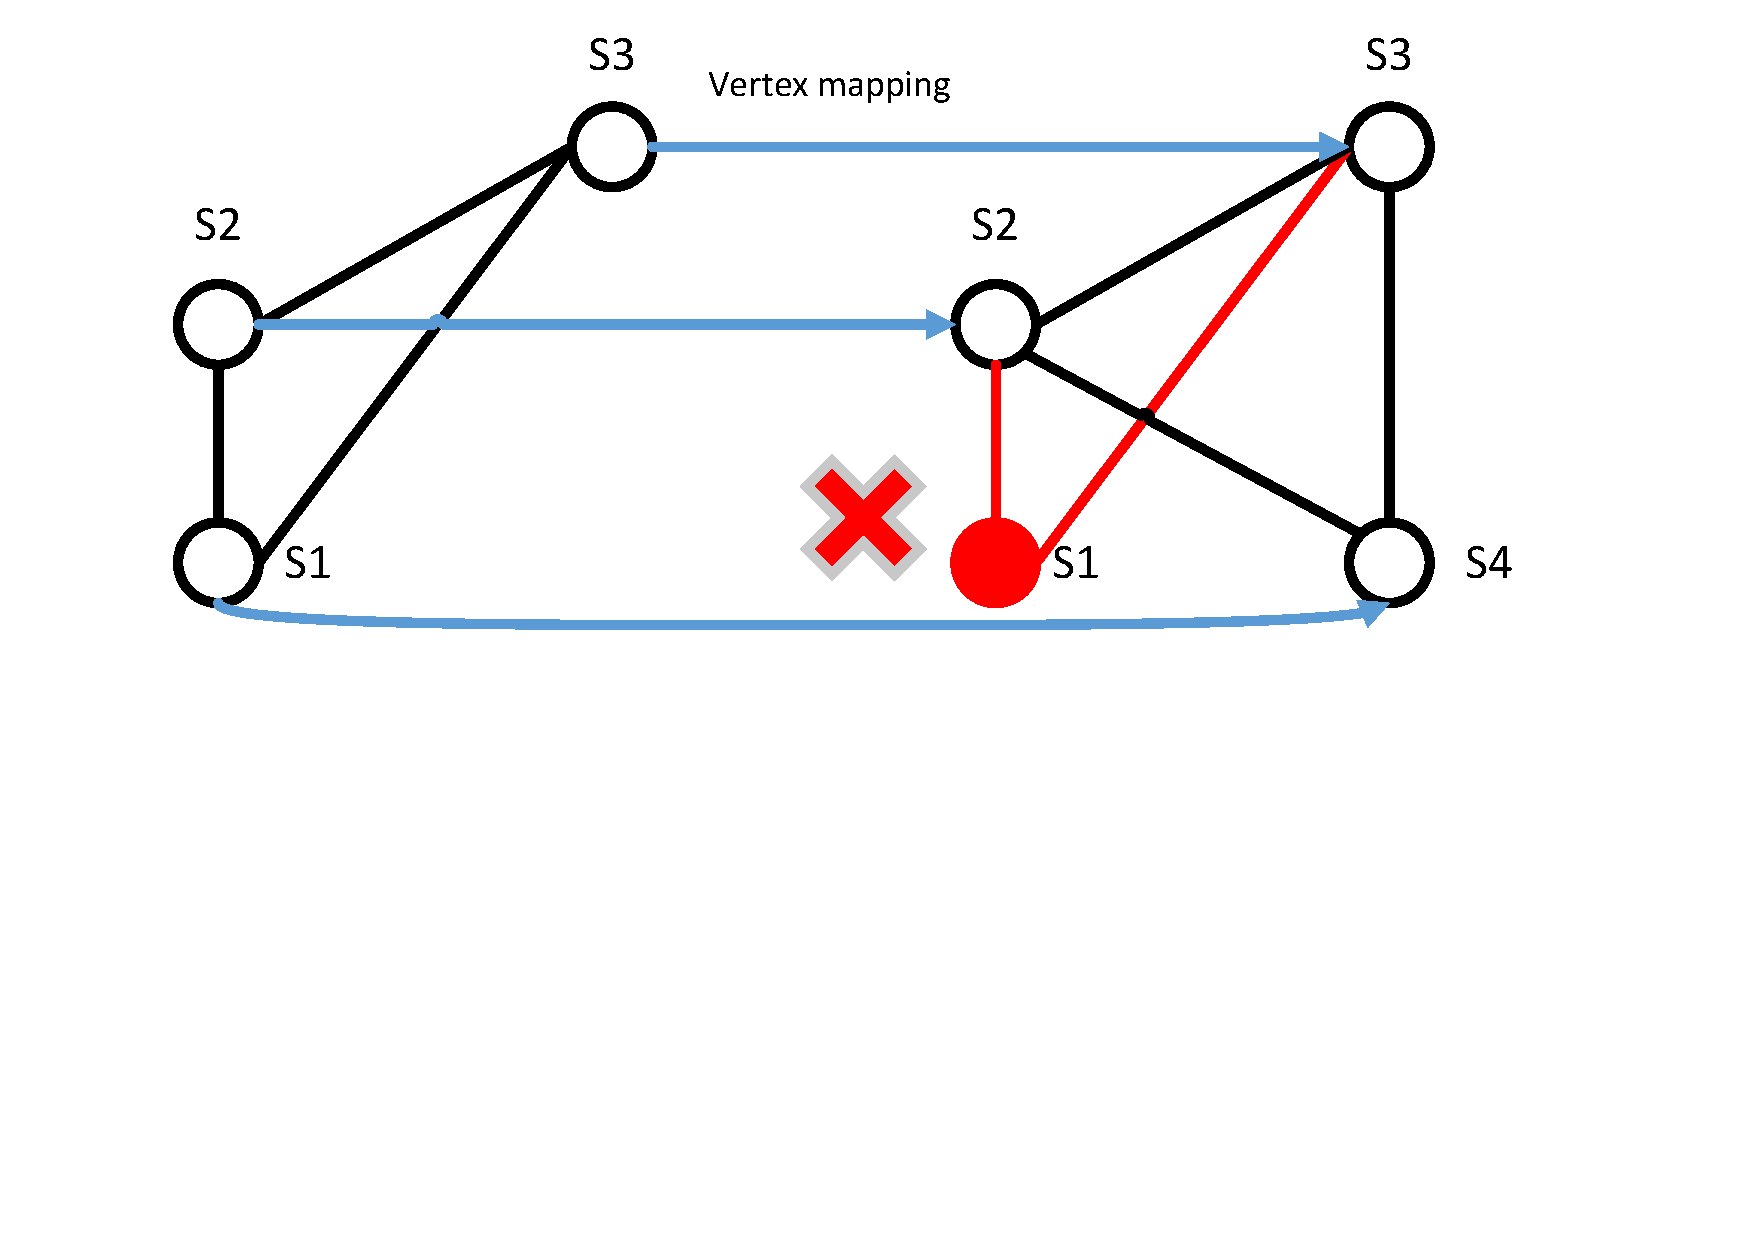
\includegraphics[width=2in]{Fig/Mapping}\\
\caption{Mapping}\label{fig:Mapping}
\end{figure}

Given the VN request $G (V,E)$
When a node fails, we denote the added node and link physical resources
To guarantee survivable virtual network embedding when a node fails, obviously,




Given a VN request $G(V,E)$ and its embedding , computer the  minimum additional resources

Given a VN request $G(V,E)$, for each node $v_i$, denote its attached physical node as $a(v_i)$. The node resource for virtual network embeddi



On the one hand, node failures  directly. On the other hand, a failure of a physical node

 two
 Survivability is the ability of a system such as a computer or a communication network to operate correctly in the presence of faults. From these studies, we can conclude that .




Given

 One extreme case for the VN protection approach
physical node may suffer the problem of instance fail.


Given the present-day importance of communications systems and infrastructures in general, networks should be designed and operated in such a way that failures can be mitigated. Network nodes  might for instance fail , and so forth. Survivable have been used by the networking community to capture the ability of a communications system to maintain operation when confronted
with network failures.

Therefore, in this paper, we just design a single node failure situation, but we will discuss that our algorithm extend for adapting multiple node failure situation.


\subsection{Survivable}
%We define reliability as the probability that critical nodes of a VInf remain in operation, over all possible node failures. This is not to be confused with availability, which is defined as a ratio of uptime to the sum of uptime and downtime

Survivability is guaranteed on the set of critical nodes of a VN through redundant virtual nodes with backup nodes set $B(V,F)$, we suppose all virtual node as critical node in this paper. In Fig.\ref{fig:eVN}, node set $V$ of backup node $B(V,S)$ is $\{s_5,s_6,s_7\}$, function type set $F$ of node is $\{\{f_1,f_2\},\{f_1,f_4\},\{f_2,f_3\}\}$. A backup (redundant) node $b_i$ may not be able to assume full execution function of a failed critical node. Hence, the backup node may not have sufficient resources in terms of computation resource.


%\subsection{How many backups?}
%The number of backup nodes depend on the physical mapping, and the failure models of both the physical nodes and the virtual infrastructure.

%The problem is to  allocate least resources for a VN $G$, including redundancy such that a reliability guarantee of at least r is achieved.


\subsection{Survivable embedded Virtual Network Request}

In this subsection, we define the SeVN design problem as follows, for a given VN request with $|V|$ nodes, the VN had been already embedded in substrate network SN and every node running function $f_i(f_i\in F^V_i)$, protect the VN with some augmented backup nodes and a set of appropriate links to connect these virtual nodes, and reserve sufficient computing and communication resources in these nodes and links to guarantee the restorability of VN request after a facility/substrate node failure.

There are different combinations of function type with respect to  every nodes of embedded virtual network, but there is only one type of function type running onto substrate node which corresponding one embedded virtual node at one moment.

There exist many backup virtual nodes $B(V,S)$ which are abstracted from un-startup substrate network's node. When one fault node $v_i$ appeared in virtual network request $G^V (V^V,E^V,f^V,C^V,B^V)$, Solving the survivable request of embedded virtual network is of approximately equivalence with asking 1-FNFT$(G,B)$ of graph $G$ and backup nodes set $B$ without computation and bandwidth's limitation.

There exist popular and easy to understand method\cite{yeow2011designing} as show in Fig.\ref{fig:FI}, when every virtual nodes fail iteratively because the corresponding the failure substrate node occur failure, then directly startup new node, connect link among nodes $V\cup B$, augment node computing or augment demand bandwidth of existing link as shown in \ref{fig:FI}. The rude method demand startup 4 new nodes, 8 new edges, 16 node computing and 36 edge bandwidth.

After a failure, even an unaffected virtual node may be migrated from a working host node to its corresponding backup host node, the former method\cite{yeow2011designing} do not consider the situation of node's migration.


We supposed a novel method STAR algorithm, which augment resource as shown in Fig.\ref{fig:FD}, our method demand startup 2 new nodes, 5 new edges, 11 node computing and 23 edge bandwidth.

\begin{figure}
\centering
\begin{minipage}[t]{0.4\linewidth}
\centering
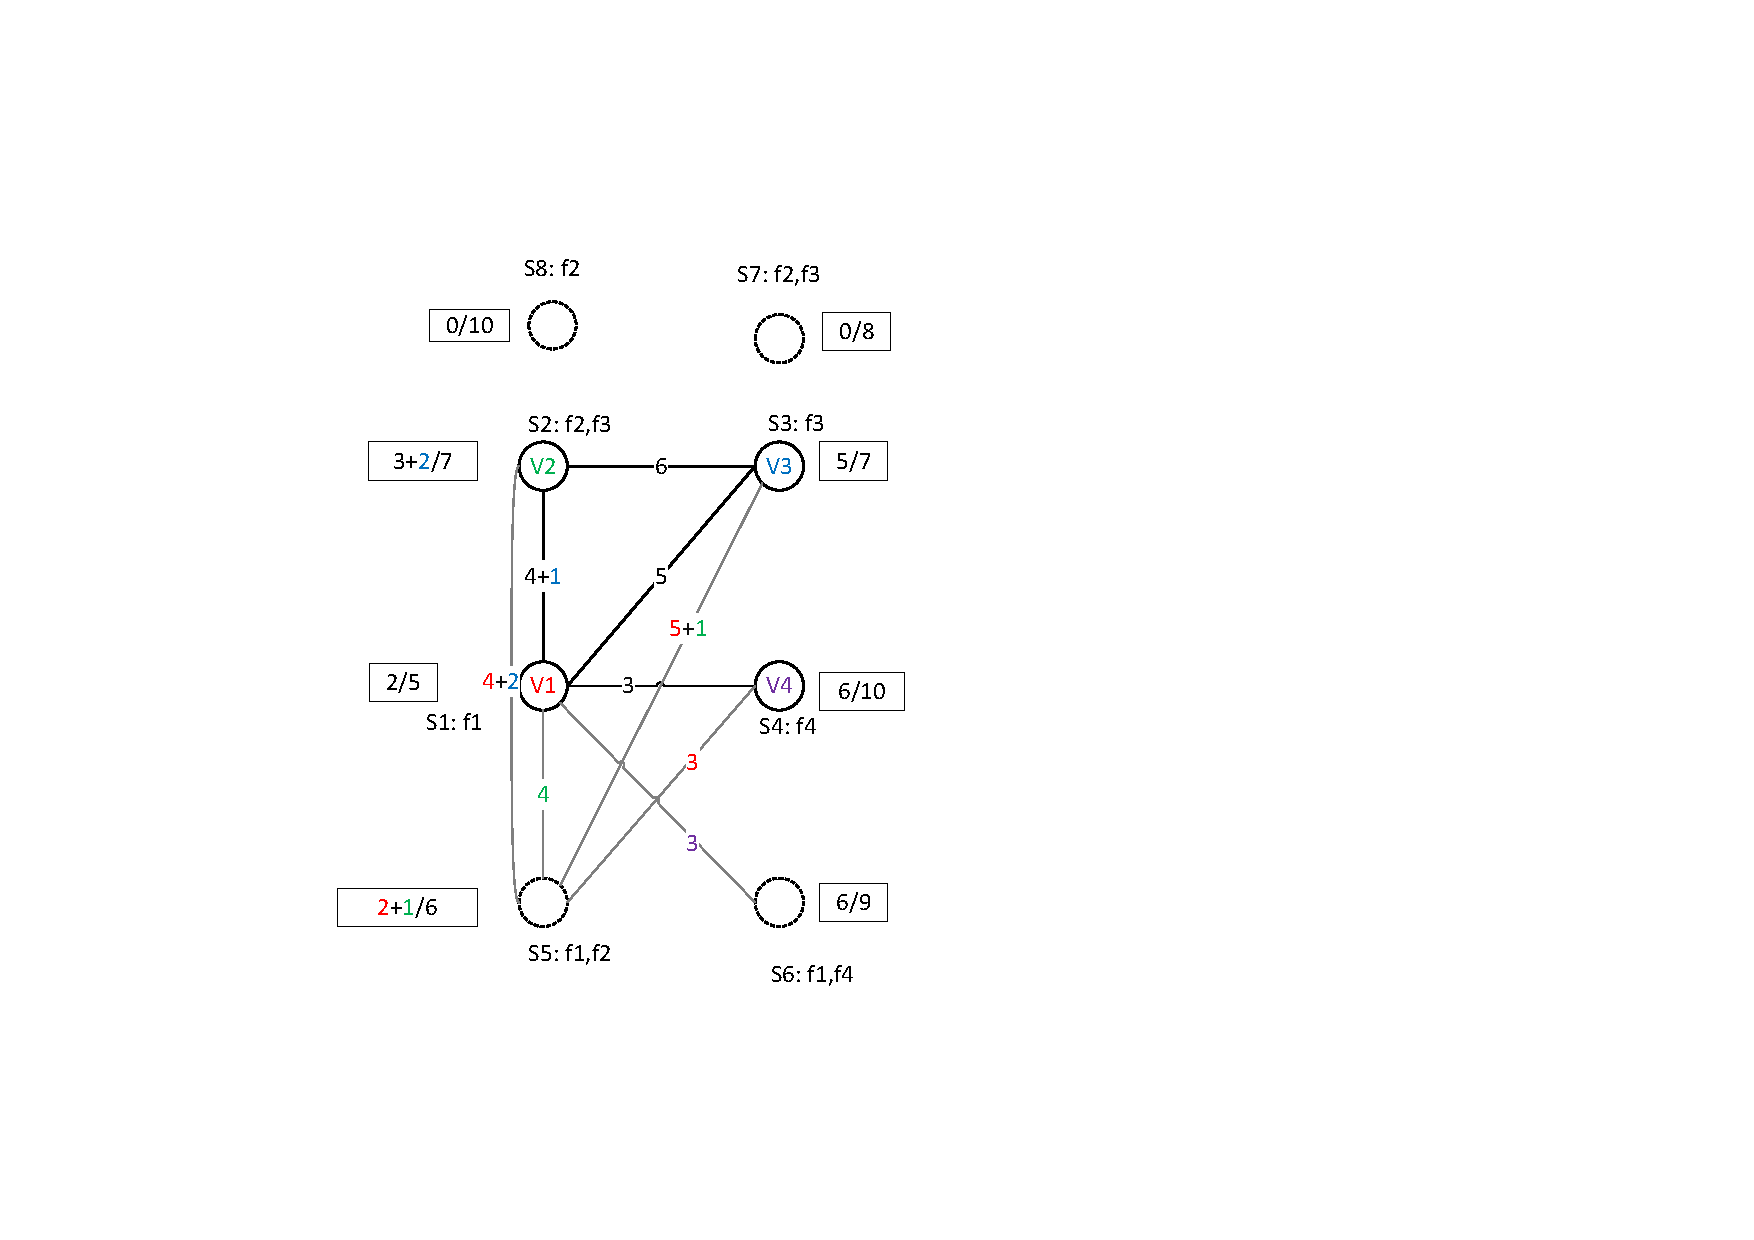
\includegraphics[width=1.5in]{Fig/FD}\\
\caption{ FD}\label{fig:FD}
\end{minipage}
\hfill
\begin{minipage}[t]{0.4\linewidth}
\centering
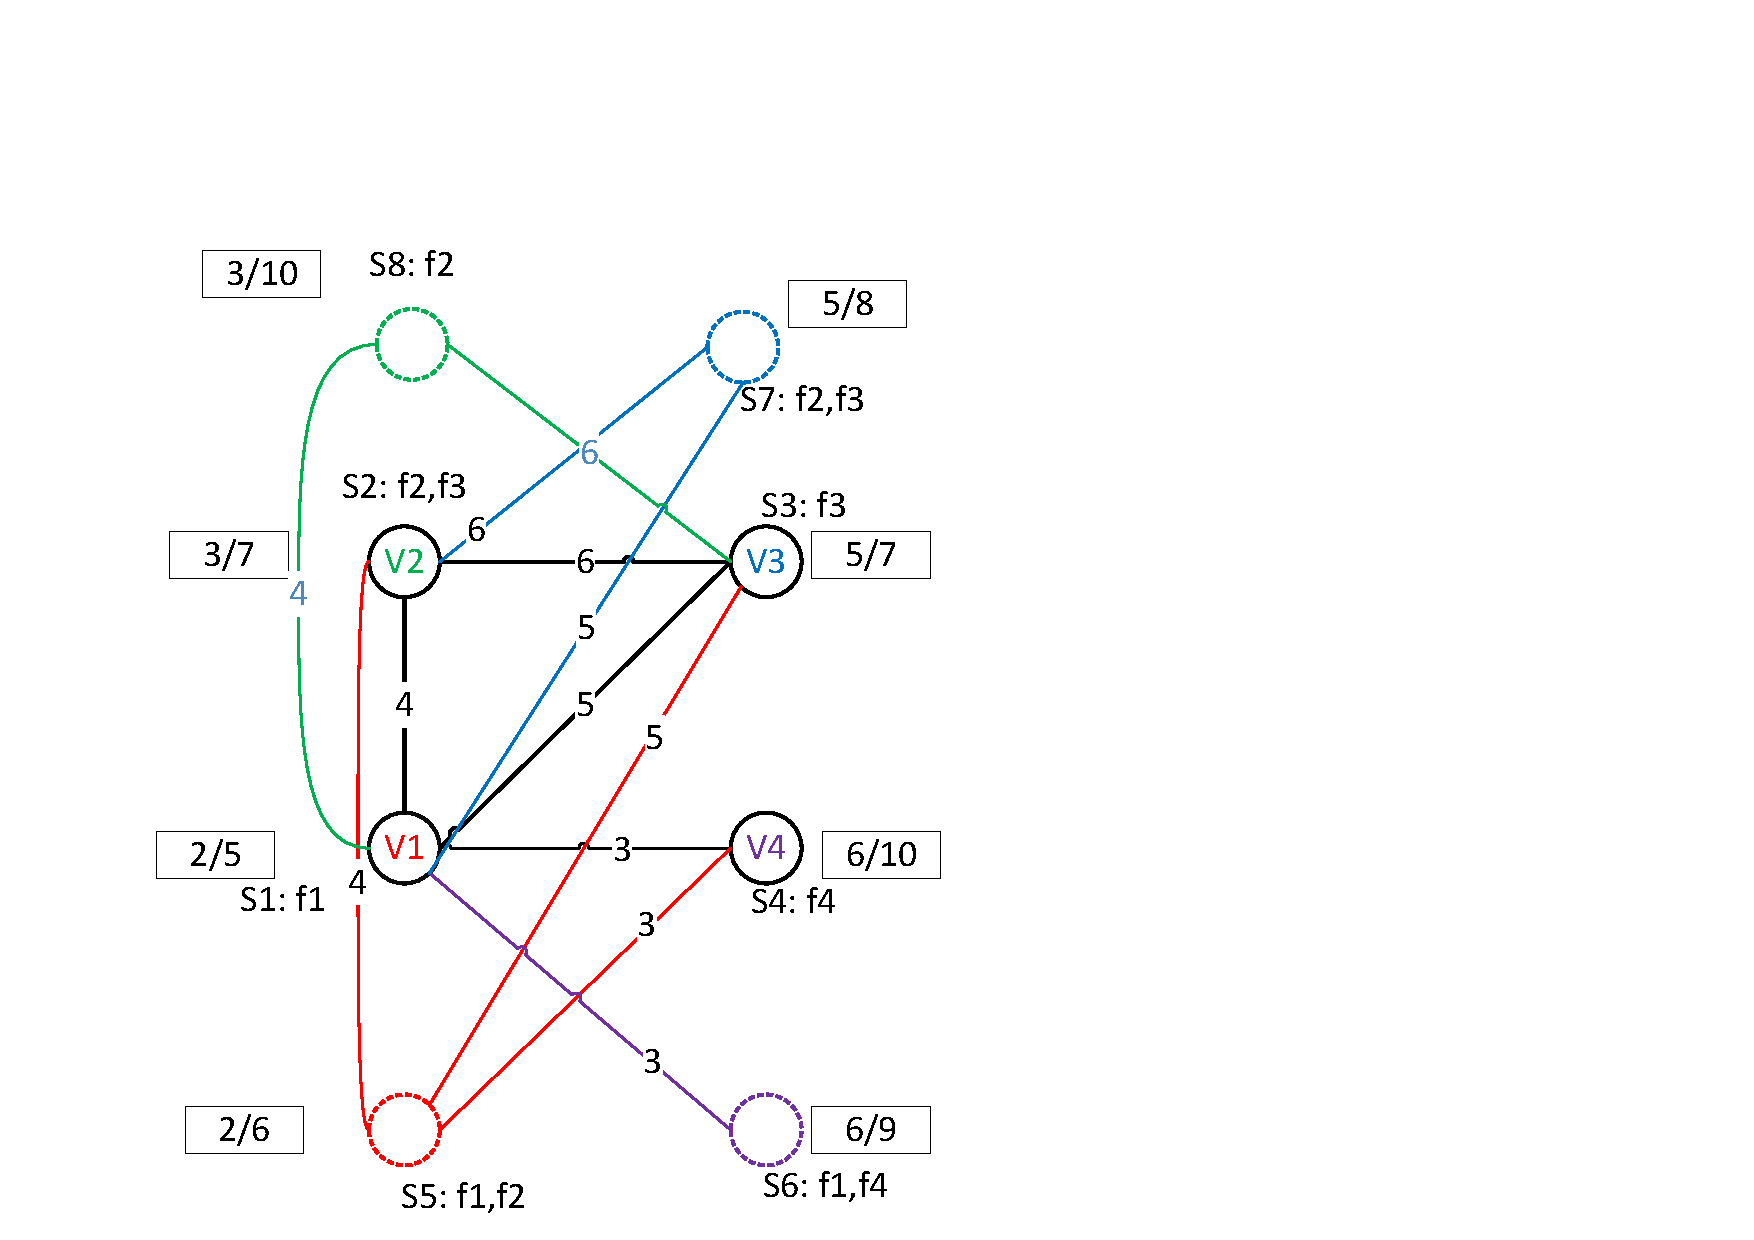
\includegraphics[width=1.5in]{Fig/FI}\\
\caption{FI}\label{fig:FI}
\end{minipage}
\end{figure}




There exist many approaches is modeled as the VN embedding (VNE) problem which attracts a broad interest recently\cite{fischer2013virtual}. VNE is extremely important in order to maximize the number of coexisting VNs and increase the utilization of substrate infrastructures. Virtual Network Embedding deals with the allocation of virtual resources both in nodes and links. Therefore, it can be divided in two sub-problems: Virtual Node Mapping (VNoM) where virtual nodes have to be allocated in physical nodes and Virtual Link Mapping (VLiM) where virtual links connecting these virtual nodes have to be mapped to paths connecting the
corresponding nodes in the substrate network. There has existed most studies about virtual network embedding method listed in a survey paper\cite{fischer2013virtual}. After all, we randomly choose a virtual network embedding method with considering three constraints: node computing, edge bandwidth and node function type from existed virtual network embedding method. As shown in Fig.\ref{fig:VNmapSN}(a), we embed virtual network request as shown in Fig.\ref{fig:VNQ} into the substrate network, node $v_1$ is embedded in node $s_1$, node $v_2$ is embedded in node $s_2$, node $v_3$ is embedded in node $s_3$, node $v_4$ is embedded in node $s_4$. demand node computing of every virtual node is not more than these virtual nodes corresponding substrate node's remain node computing. Every link of virtual network request exist a corresponding path consisted of substrate node and remain bandwidth of all links of corresponding path is more than demand  bandwidth of the virtual network link.


\subsection{Embedded Virtual Network}
\label{sec:embeddedVirtualNetwork}
When a virtual network request has been inserted in to substrate network, augmented resource is attached into virtual network, embedded virtual network denote as $G^V (V^V,E^V,f^V,F^V,C^V,B^V,M^V)$ as shown in Fig.\ref{fig:eVN}. $F^V$ denote a set of function type set $F^V_i$($f^V_i\in F^V_i$) which corresponding to every VN nodes $v_i$. $C^V$ denote node's computational resource's capacity. $B^V$ denote edge's bandwidth resource's capacity. $M^V$ denote node's mapping relationship of virtual network embedding algorithm, $M_{i}=j$ represent that the i-th VN's node had been embedded at j-th substrate network node. Besides, with respect to the node embedding, we suppose a assumption that all virtual nodes of VN should be mapped on isolated physically substrate nodes.
\begin{figure}
\centering
% Requires \usepackage{graphicx}
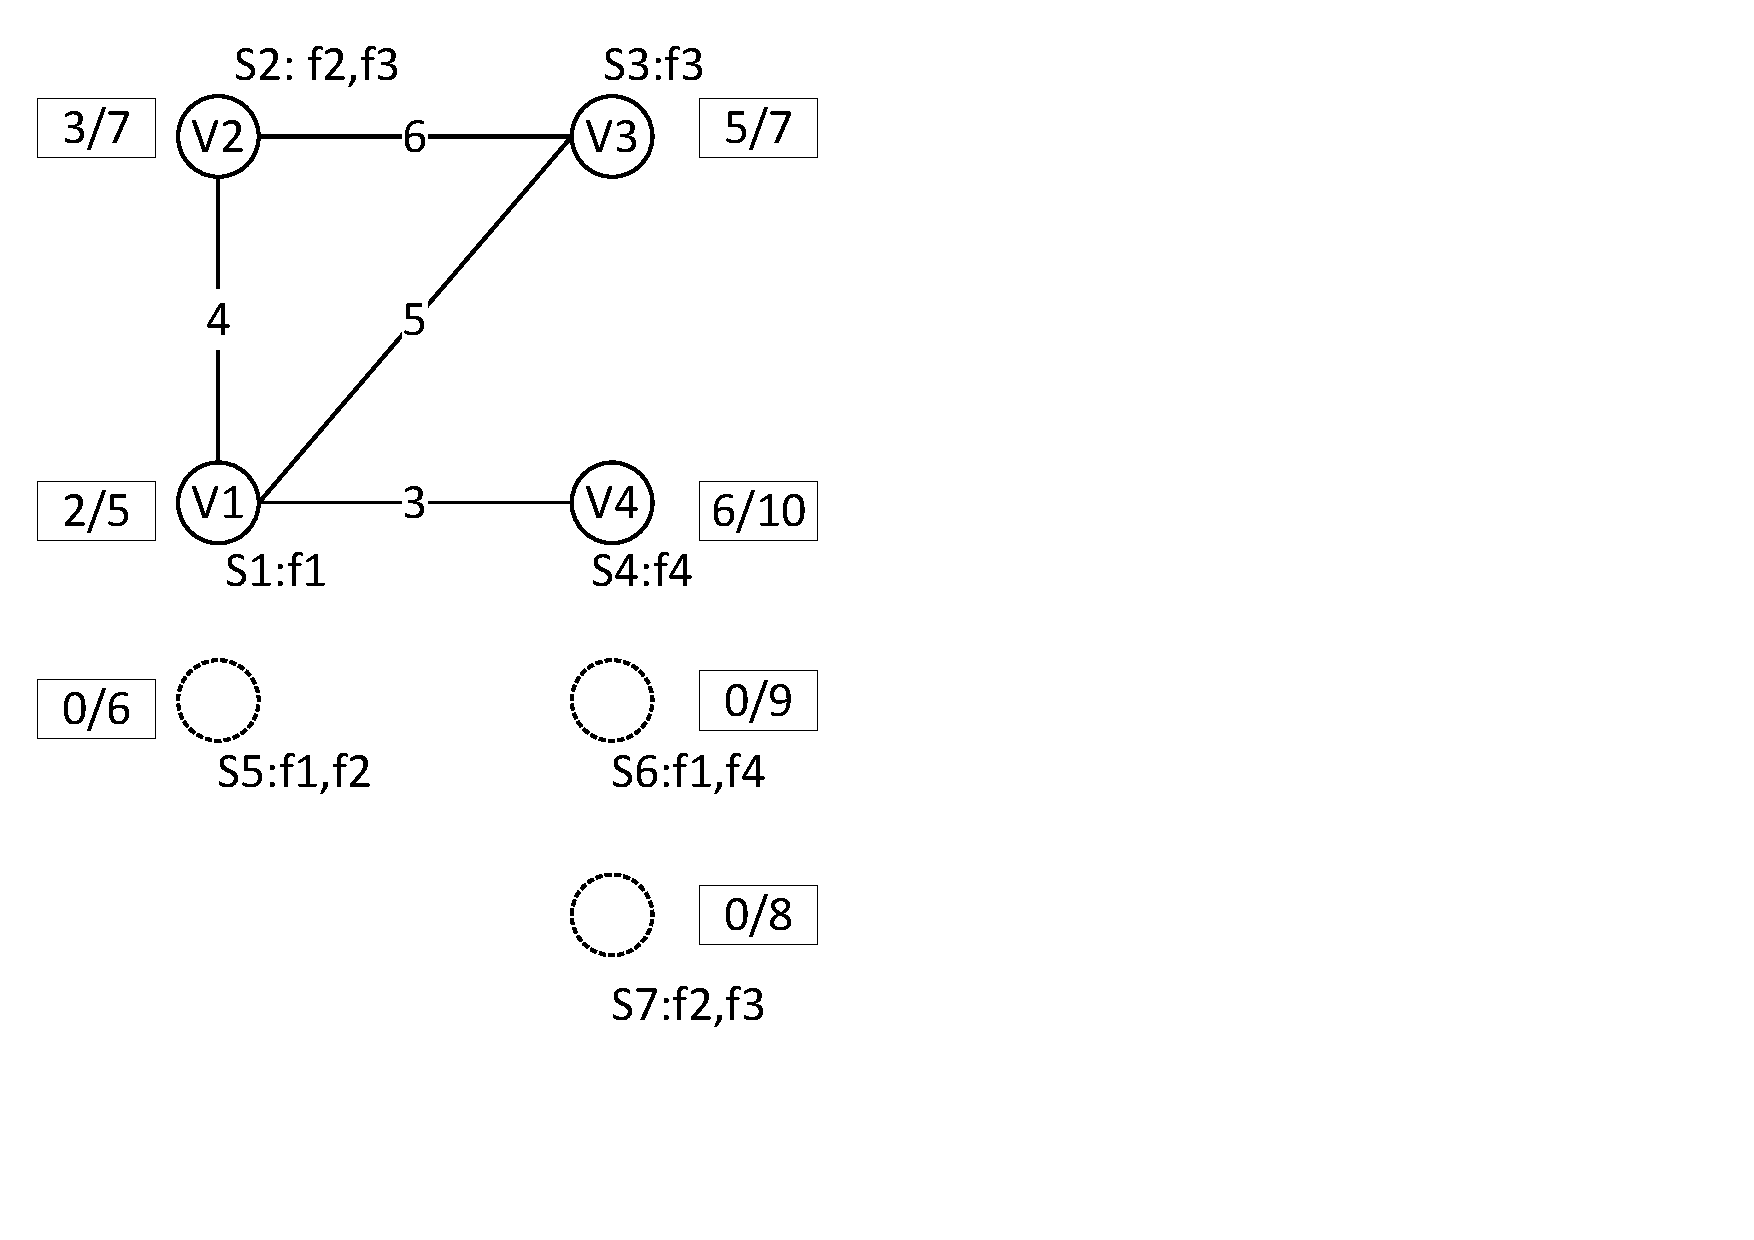
\includegraphics[width=2in]{Fig/eVN}\\
\caption{embedded Virtual Network $G^V (V^V,E^V,f^V,F^V,C^V,B^V,M^V_V)$, $V^V:\{s_1,s_2,s_3,s_4,s_5,s_6,s_7\}$, $E^V=\{e_{12},e_{23},e_{13},e_{14}\}$, $f^V:\{f_1,f_2,f_3,f_4\}$,
$F^V=\{\{f_1\},\{f_2,f_3\},\{f_3\},\{f_4\},\{f_1,f_2\},\{f_1,f_4\},\{f_2,f_3\}\}$, $C^V=\{5,7,7,10,6,9,8\}$, $B^V=\{4,6,5,3\}$, $M^V=\{s_1,s_2,s_3,s_4\}$}\label{fig:eVN}
\end{figure}


\subsection{Node Failure}
Given the present-day importance of communications systems and infrastructures in general, networks should be designed and operated in such a way that failures can be mitigated. Network nodes  might for instance fail due to malicious attacks, natural disasters, unintentional cable cuts, planned maintenance, equipment malfunctioning, and so forth. Survivable have been used by the networking community to capture the ability of a communications system to maintain operation when confronted
with network failures.

In general, the substrate nodes simultaneous failure is mutual independent , a single node failure happen at most of time\cite{yeow2011designing}. Therefore, in this paper, we just design a single node failure situation, but we will discuss that our algorithm extend for adapting multiple node failure situation.


\subsection{Survivable}
%We define reliability as the probability that critical nodes of a VInf remain in operation, over all possible node failures. This is not to be confused with availability, which is defined as a ratio of uptime to the sum of uptime and downtime

Survivability is guaranteed on the set of critical nodes of a VN through redundant virtual nodes with backup nodes set $B(V,F)$, we suppose all virtual node as critical node in this paper. In Fig.\ref{fig:eVN}, node set $V$ of backup node $B(V,S)$ is $\{s_5,s_6,s_7\}$, function type set $F$ of node is $\{\{f_1,f_2\},\{f_1,f_4\},\{f_2,f_3\}\}$. A backup (redundant) node $b_i$ may not be able to assume full execution function of a failed critical node. Hence, the backup node may not have sufficient resources in terms of computation resource.


%\subsection{How many backups?}
%The number of backup nodes depend on the physical mapping, and the failure models of both the physical nodes and the virtual infrastructure.

%The problem is to  allocate least resources for a VN $G$, including redundancy such that a reliability guarantee of at least r is achieved.


\subsection{Survivable embedded Virtual Network Request}

In this subsection, we define the SeVN design problem as follows, for a given VN request with $|V|$ nodes, the VN had been already embedded in substrate network SN and every node running function $f_i(f_i\in F^V_i)$, protect the VN with some augmented backup nodes and a set of appropriate links to connect these virtual nodes, and reserve sufficient computing and communication resources in these nodes and links to guarantee the restorability of VN request after a facility/substrate node failure.

There are different combinations of function type with respect to  every nodes of embedded virtual network, but there is only one type of function type running onto substrate node which corresponding one embedded virtual node at one moment.

There exist many backup virtual nodes $B(V,S)$ which are abstracted from un-startup substrate network's node. When one fault node $v_i$ appeared in virtual network request $G^V (V^V,E^V,f^V,C^V,B^V)$, Solving the survivable request of embedded virtual network is of approximately equivalence with asking 1-FNFT$(G,B)$ of graph $G$ and backup nodes set $B$ without computation and bandwidth's limitation.

There exist popular and easy to understand method\cite{yeow2011designing} as show in Fig.\ref{fig:FI}, when every virtual nodes fail iteratively because the corresponding the failure substrate node occur failure, then directly startup new node, connect link among nodes $V\cup B$, augment node computing or augment demand bandwidth of existing link as shown in \ref{fig:FI}. The rude method demand startup 4 new nodes, 8 new edges, 16 node computing and 36 edge bandwidth.

After a failure, even an unaffected virtual node may be migrated from a working host node to its corresponding backup host node, the former method\cite{yeow2011designing} do not consider the situation of node's migration.


We supposed a novel method STAR algorithm, which augment resource as shown in Fig.\ref{fig:FD}, our method demand startup 2 new nodes, 5 new edges, 11 node computing and 23 edge bandwidth.

\begin{figure}
\centering
\begin{minipage}[t]{0.4\linewidth}
\centering
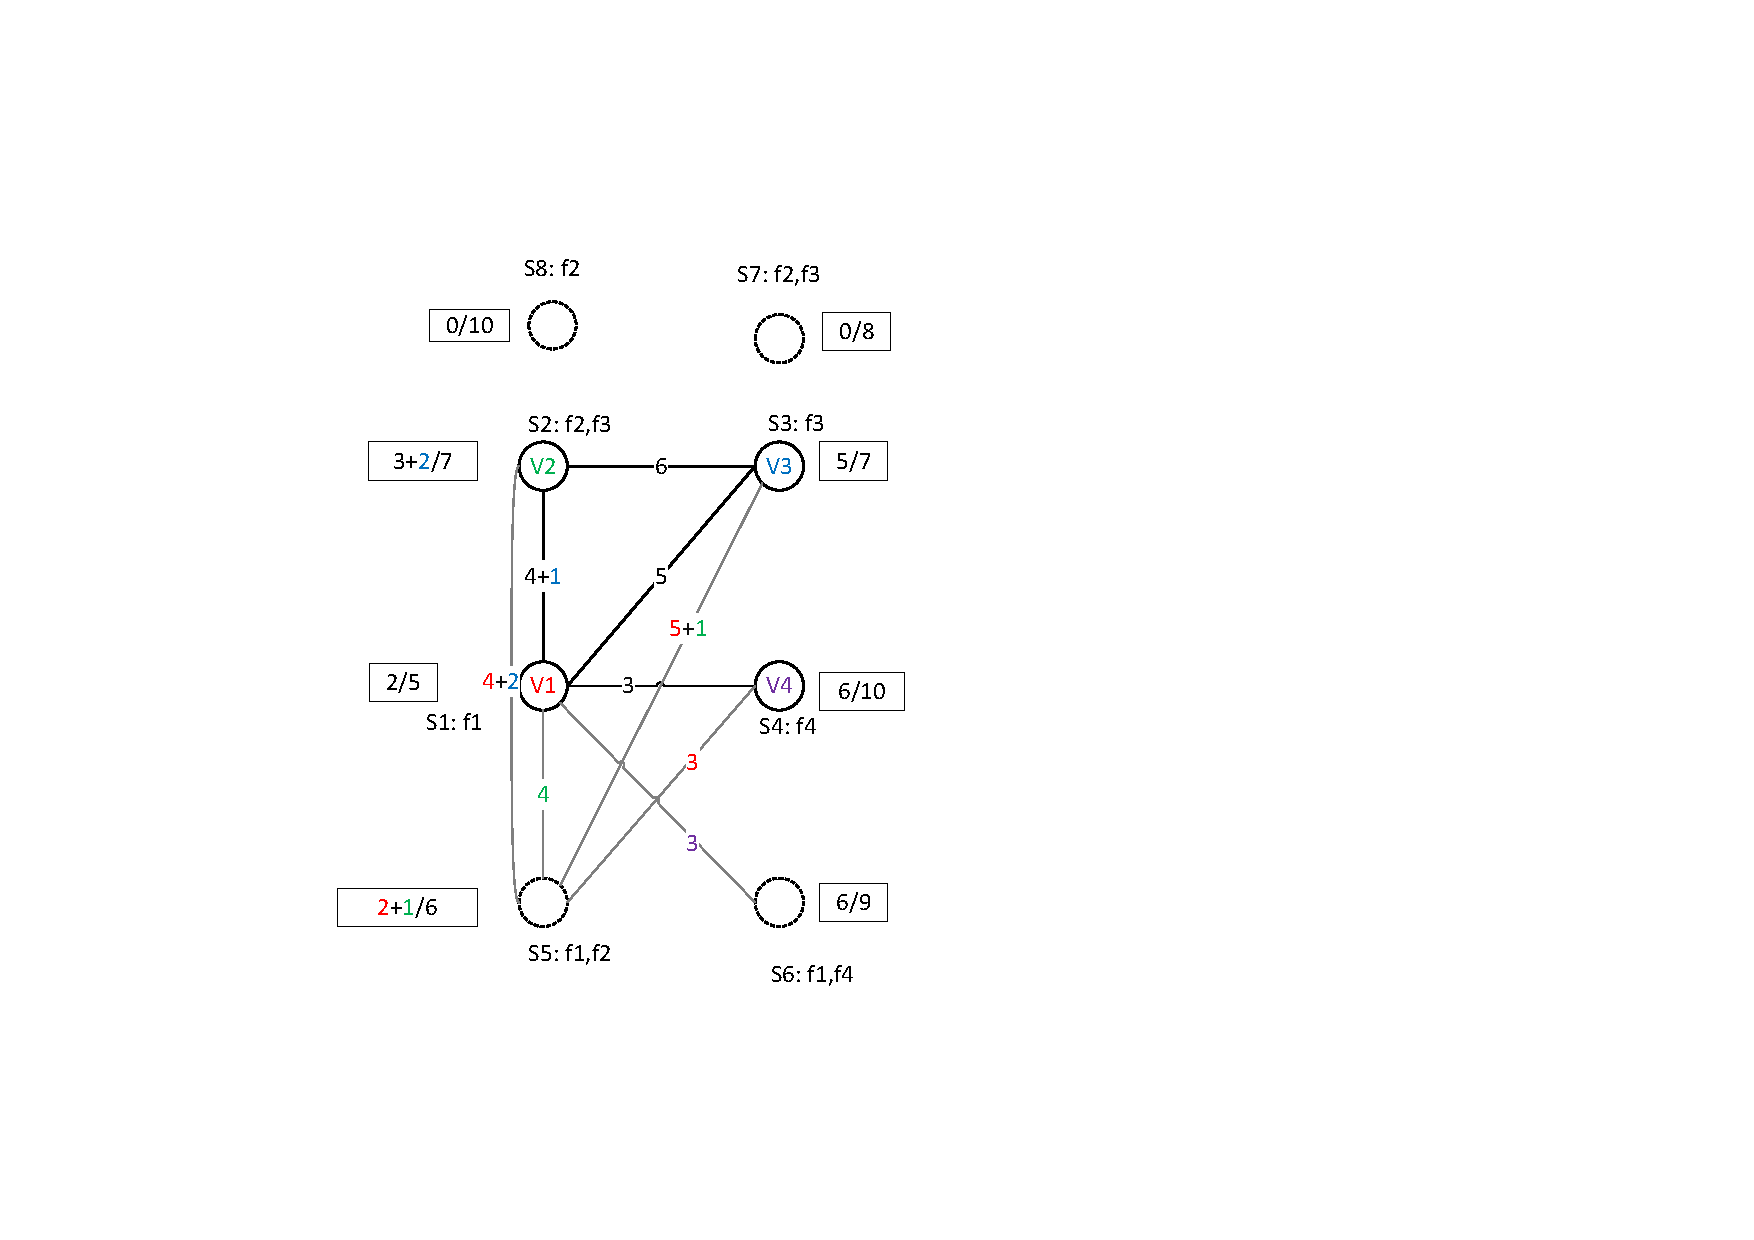
\includegraphics[width=1.8in]{Fig/FD}\\
\caption{ $\MyAlgorithmMethodAbrreviation$ algorithm protection scheme}\label{fig:FD}
\end{minipage}
\hfill
\begin{minipage}[t]{0.4\linewidth}
\centering
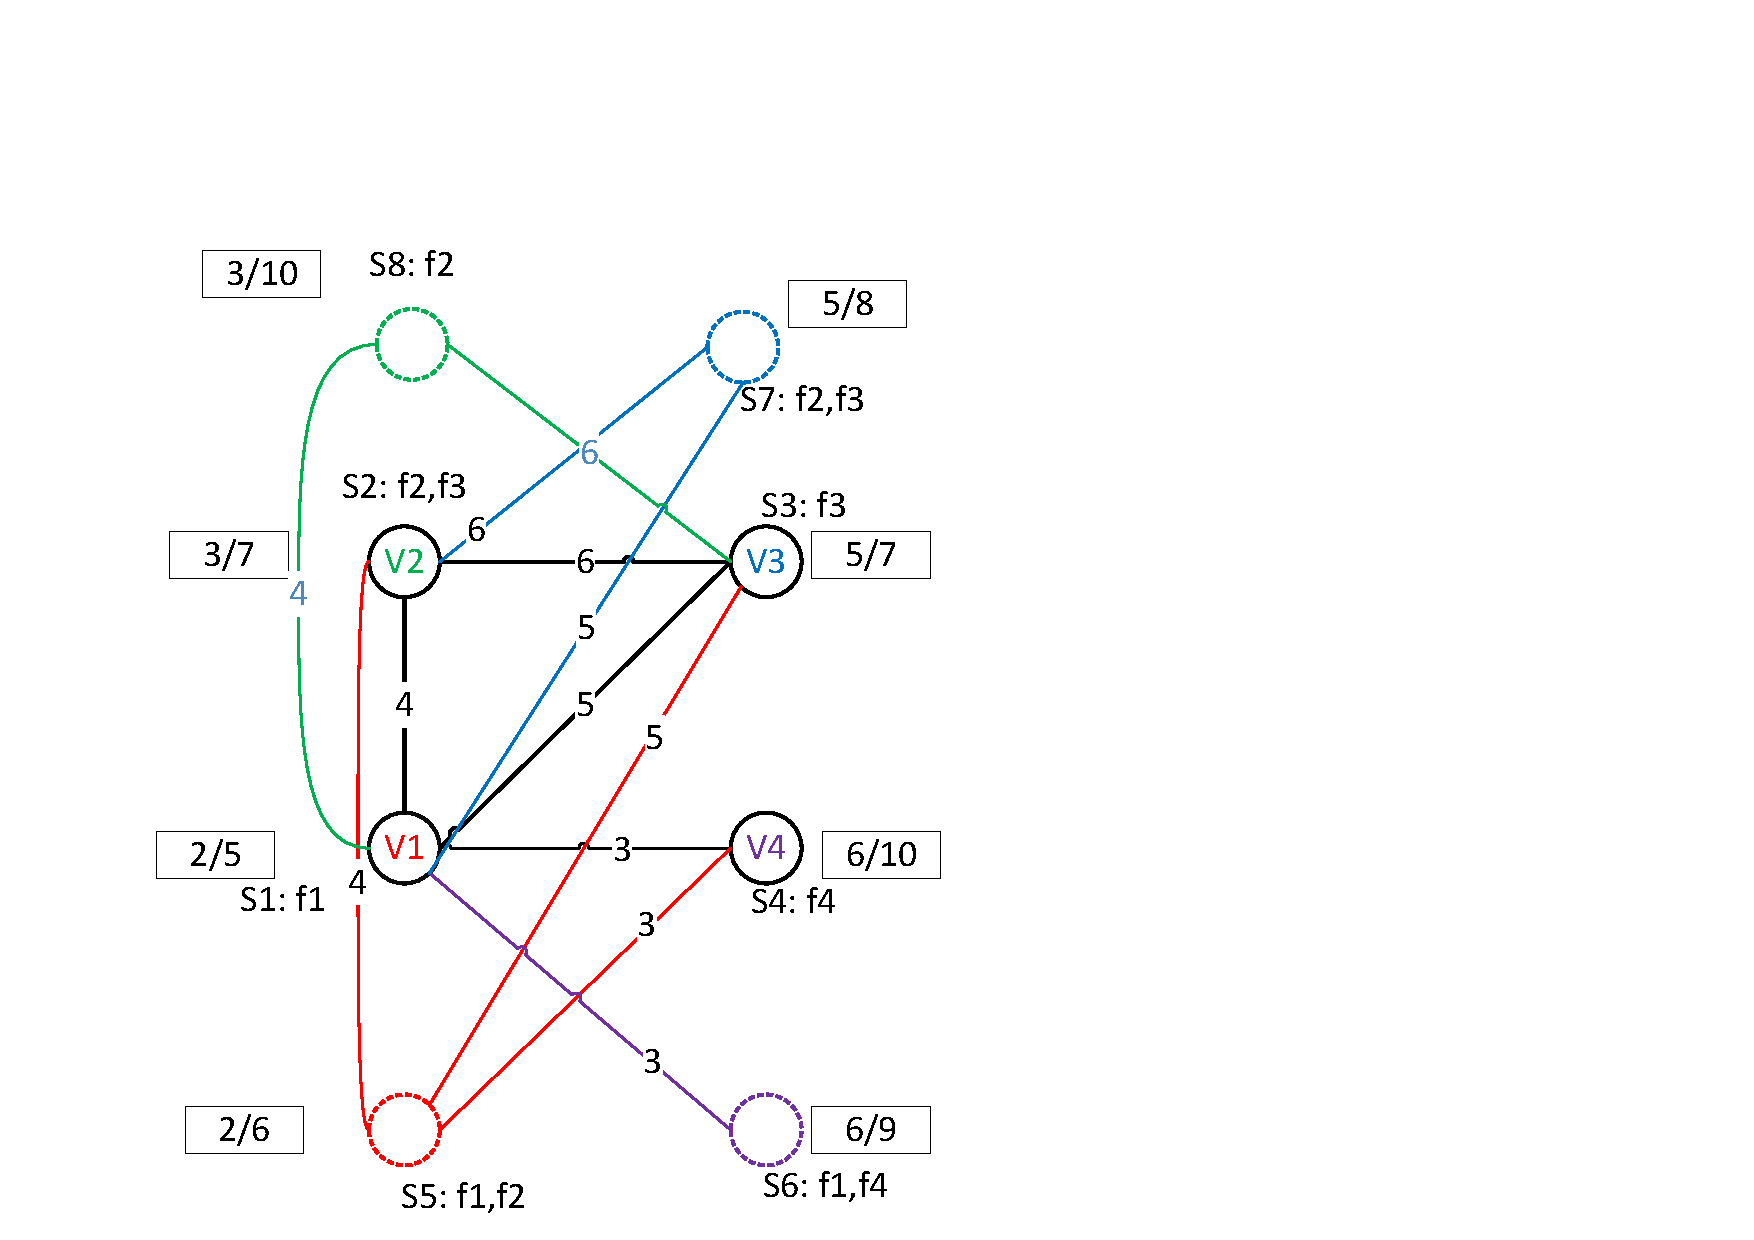
\includegraphics[width=1.8in]{Fig/FI}\\
\caption{1+1-protection scheme}\label{fig:FI}
\end{minipage}
\end{figure}


